% move all configuration stuff into one file so we can focus on the content
\documentclass[aspectratio=169,hyperref={pdfpagelabels=false,colorlinks=true,linkcolor=white,urlcolor=lightblue},xcolor={table},t]{beamer}

%%%%%%%%%%%%%%%%%%%%%%%%%%%%%%%%%%%%%%%%%%%%%%%%%%%%%%%%%%%%%%%%%%%%%%%%%%%%%%%%%%
%%%%%%%%%%%%%%%%%%%%%%%%%%%%%%%%%%%%%%%%%%%%%%%%%%%%%%%%%%%%%%%%%%%%%%%%%%%%%%%%%%
% packages
\usepackage{pict2e}
\usepackage{epic}
\usepackage{amsmath,amsfonts,amssymb}
\usepackage{units}
\usepackage{fancybox}
\usepackage[absolute,overlay]{textpos} 
%\usepackage[table]{xcolor}
\usepackage{animate}
\usepackage{gensymb}
%\usepackage{graphicx}
%\usepackage{longtable}
\usepackage{multirow}
\usepackage{silence}
\usepackage{tikz}
\usepackage[backend=bibtex,style=ieee]{biblatex}
\AtEveryCitekey{\iffootnote{\tiny}{}}
%\addbibresource{include/references}



% fontsize
\let\Tiny=\tiny

%%%%%%%%%%%%%%%%%%%%%%%%%%%%%%%%%%%%%%%%%%%%%%%%%%%%%%%%%%%%%%%%%%%%%%%%%%%%%%%%%%
%%%%%%%%%%%%%%%%%%%%%%%%%%%%%%%%%%%%%%%%%%%%%%%%%%%%%%%%%%%%%%%%%%%%%%%%%%%%%%%%%%
% warnings
\pdfsuppresswarningpagegroup=1
\WarningFilter{biblatex}{Patching footnotes failed}
\WarningFilter{latexfont}{Font shape}
\WarningFilter{latexfont}{Some font shapes}
\WarningFilter{gensymb}{Not defining}


%%%%%%%%%%%%%%%%%%%%%%%%%%%%%%%%%%%%%%%%%%%%%%%%%%%%%%%%%%%%%%%%%%%%%%%%%%%%%%%%%%
%%%%%%%%%%%%%%%%%%%%%%%%%%%%%%%%%%%%%%%%%%%%%%%%%%%%%%%%%%%%%%%%%%%%%%%%%%%%%%%%%%
% colors
\definecolor{gtgold}{rgb}{.914, .664, 0} %0e7eed {rgb}{0.88,0.66,1,0.06} [234, 170, 0]/256 %96caff
\definecolor{darkgray}{rgb}{.15, .15, .15}
\definecolor{lightblue}{HTML}{0e7eed}
\definecolor{highlight}{rgb}{0, 0, 1} %_less!40

%%%%%%%%%%%%%%%%%%%%%%%%%%%%%%%%%%%%%%%%%%%%%%%%%%%%%%%%%%%%%%%%%%%%%%%%%%%%%%%%%%
%%%%%%%%%%%%%%%%%%%%%%%%%%%%%%%%%%%%%%%%%%%%%%%%%%%%%%%%%%%%%%%%%%%%%%%%%%%%%%%%%%
% relative paths
\graphicspath{{../graph/}}


%%%%%%%%%%%%%%%%%%%%%%%%%%%%%%%%%%%%%%%%%%%%%%%%%%%%%%%%%%%%%%%%%%%%%%%%%%%%%%%%%%
%%%%%%%%%%%%%%%%%%%%%%%%%%%%%%%%%%%%%%%%%%%%%%%%%%%%%%%%%%%%%%%%%%%%%%%%%%%%%%%%%%
% units
\setlength{\unitlength}{1mm}

%%%%%%%%%%%%%%%%%%%%%%%%%%%%%%%%%%%%%%%%%%%%%%%%%%%%%%%%%%%%%%%%%%%%%%%%%%%%%%%%%%
%%%%%%%%%%%%%%%%%%%%%%%%%%%%%%%%%%%%%%%%%%%%%%%%%%%%%%%%%%%%%%%%%%%%%%%%%%%%%%%%%%
% math
\DeclareMathOperator*{\argmax}{argmax}
\DeclareMathOperator*{\argmin}{argmin}
\DeclareMathOperator*{\atan}{atan}
\DeclareMathOperator*{\arcsinh}{arcsinh}
\DeclareMathOperator*{\sign}{sign}
\DeclareMathOperator*{\tcdf}{tcdf}
\DeclareMathOperator*{\si}{sinc}
\DeclareMathOperator*{\princarg}{princarg}
\DeclareMathOperator*{\arccosh}{arccosh}
\DeclareMathOperator*{\hwr}{HWR}
\DeclareMathOperator*{\flip}{flip}
\DeclareMathOperator*{\sinc}{sinc}
\DeclareMathOperator*{\floor}{floor}
\newcommand{\e}{{e}}
\newcommand{\jom}{\mathrm{j}\omega}
\newcommand{\jOm}{\mathrm{j}\Omega}
\newcommand   {\mat}[1]    		{\boldsymbol{\uppercase{#1}}}		%bold
\renewcommand {\vec}[1]    		{\boldsymbol{\lowercase{#1}}}		%bold

%%%%%%%%%%%%%%%%%%%%%%%%%%%%%%%%%%%%%%%%%%%%%%%%%%%%%%%%%%%%%%%%%%%%%%%%%%%%%%%%%%
%%%%%%%%%%%%%%%%%%%%%%%%%%%%%%%%%%%%%%%%%%%%%%%%%%%%%%%%%%%%%%%%%%%%%%%%%%%%%%%%%%
% media9
\newcommand{\includeaudio}[1]{
\href{run:audio/#1.mp3}{
\includegraphics[width=5mm, height=5mm]{graph/SpeakerIcon}}}

\newcommand{\includeanimation}[4]{{\begin{center}
                        \animategraphics[autoplay,loop,scale=.7]{#4}{animation/#1-}{#2}{#3}        
                        \end{center}
                        \addreference{matlab source: \href{https://github.com/alexanderlerch/ACA-Plots/blob/master/matlab/animate#1.m}{matlab/animate#1.m}}}
                        \inserticon{video}}
                        
%%%%%%%%%%%%%%%%%%%%%%%%%%%%%%%%%%%%%%%%%%%%%%%%%%%%%%%%%%%%%%%%%%%%%%%%%%%%%%%%%%
%%%%%%%%%%%%%%%%%%%%%%%%%%%%%%%%%%%%%%%%%%%%%%%%%%%%%%%%%%%%%%%%%%%%%%%%%%%%%%%%%%
% other commands
\newcommand{\question}[1]{%\vspace{-4mm}
                          \setbeamercovered{invisible}
                          \begin{columns}[T]
                            \column{.9\textwidth}
                                \textbf{#1}
                            \column{.1\textwidth}
                                \vspace{-8mm}
                                \begin{flushright}
                                     
\includegraphics[width=.9\columnwidth]{graph/question_mark}
                                \end{flushright}
                                \vspace{6mm}
                          \end{columns}\pause\vspace{-12mm}}

\newcommand{\toremember}[1]{
                        \inserticon{lightbulb}
                        }

\newcommand{\matlabexercise}[1]{%\vspace{-4mm}
                          \setbeamercovered{invisible}
                          \begin{columns}[T]
                            \column{.8\textwidth}
                                \textbf{matlab exercise}: #1
                            \column{.2\textwidth}
                                \begin{flushright}
                                     \includegraphics[scale=.5]{graph/logo_matlab}
                                \end{flushright}
                                %\vspace{6mm}
                          \end{columns}}

\newcommand{\addreference}[1]{  
                  
                    \begin{textblock*}{\baselineskip }(.98\paperwidth,.5\textheight) %(1.15\textwidth,.4\textheight)
                         \begin{minipage}[b][.5\paperheight][b]{1cm}%
                            \vfill%
                             \rotatebox{90}{\tiny {#1}}
                        \end{minipage}
                   \end{textblock*}
                    }
                    
\newcommand{\figwithmatlab}[1]{
                    \begin{figure}
                        \centering
                        \includegraphics[scale=.7]{#1}
                        %\label{fig:#1}
                    \end{figure}
                    
                    \addreference{matlab source: \href{https://github.com/alexanderlerch/MUSI-6202/blob/main/matlab/plot#1.m}{plot#1.m}}}
\newcommand{\figwithref}[2]{
                    \begin{figure}
                        \centering
                        \includegraphics[scale=.7]{#1}
                        \label{fig:#1}
                    \end{figure}
                    
                    \addreference{#2}}  
                                    
\newcommand{\inserticon}[1]{
                    \begin{textblock*}{100mm}(14.5cm,7.5cm)
                        \includegraphics[height=.8cm,keepaspectratio]{graph/#1}
                    \end{textblock*}}            

%%%%%%%%%%%%%%%%%%%%%%%%%%%%%%%%%%%%%%%%%%%%%%%%%%%%%%%%%%%%%%%%%%%%%%%%%%%%%%%%%%
%%%%%%%%%%%%%%%%%%%%%%%%%%%%%%%%%%%%%%%%%%%%%%%%%%%%%%%%%%%%%%%%%%%%%%%%%%%%%%%%%%
% counters
\newcounter{i}
\newcounter{j}
\newcounter{iXOffset}
\newcounter{iYOffset}
\newcounter{iXBlockSize}
\newcounter{iYBlockSize}
\newcounter{iYBlockSizeDiv2}
\newcounter{iXBlockSizeDiv2}
\newcounter{iDistance}

\newcommand{\IEEELink}{https://ieeexplore.ieee.org/servlet/opac?bknumber=9965970}



\subtitle{Part 27: Denoising}

%%%%%%%%%%%%%%%%%%%%%%%%%%%%%%%%%%%%%%%%%%%%%%%%%%%%%%%%%%%%%%%%%%%%%%%%%%%%
\begin{document}
    % generate title page
	\title[]{Digital Signal Processing for Music}   
\author[alexander lerch]{alexander lerch} 
%\institute{~}
%\date[Alexander Lerch]{}
\titlegraphic{\vspace{-16mm}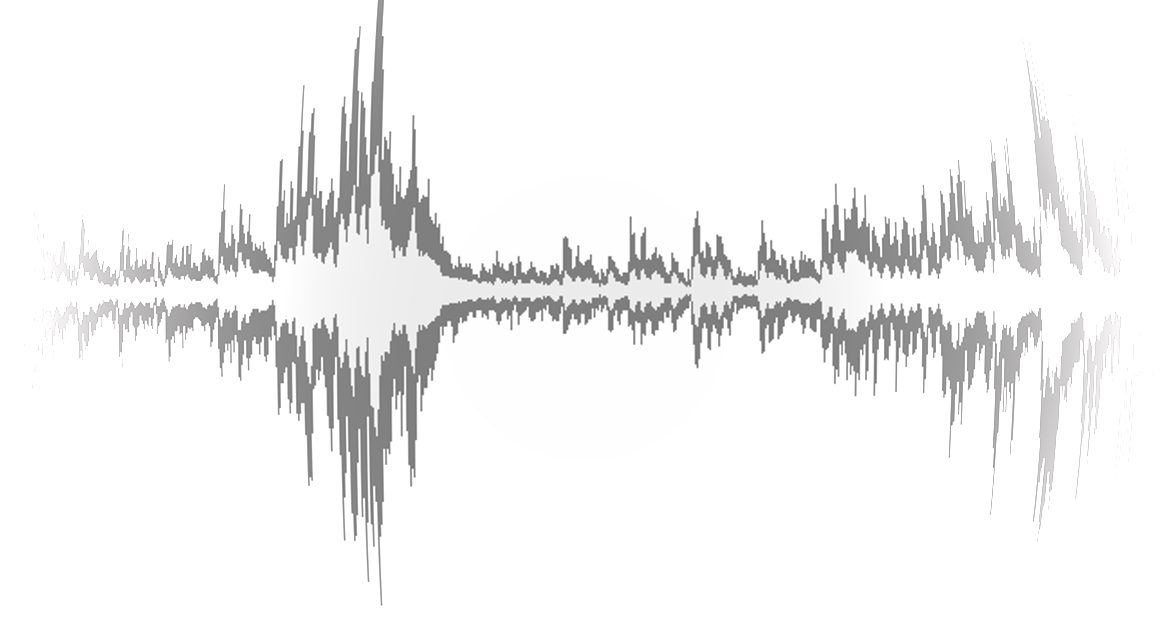
\includegraphics[width=\textwidth,height=3cm]{title}}


\begin{frame}
    \titlepage
    %\vspace{-5mm}
    \begin{flushright}
        \href{http://www.gtcmt.gatech.edu}{
\includegraphics[height=.8cm,keepaspectratio]{../shared/Logo_GTCMT_black}}
    \end{flushright}
\end{frame}


\section[intro]{introduction}
	\begin{frame}{denoising}{introduction}
		\begin{itemize}
			\item	\textbf{problem}: signal $y$ is noisy
                \begin{equation*}
                    y(i) = x(i) + n(i)                    
                \end{equation*}
            \pause
            \item   \textbf{assumptions}:
                \begin{itemize}
                    \item   noise is uncorrelated
                    \item   noise is stationary
                \end{itemize}
            \pause
            \smallskip \item   \textbf{objective}: estimate $\hat{x}$ which minimizes the error
                \begin{equation*}
                    e(i)  = x(i) - \hat{x}(i)
                \end{equation*}
            \pause
            \item   \textbf{approach}: filter the noisy signal
                \begin{equation*}
                    \hat{x}(i) = \sum\limits_{j=0}^{\mathcal{O}-1} w(j)\cdot y(i-j)
                \end{equation*}
		\end{itemize}
	\end{frame}
    \begin{frame}{denoising}{introduction 2/2}
        here: only presenting the simplest approach to noise reduction
        
        
        \pause
        \bigskip
        the \textbf{Wiener Filter}
	\end{frame}

\section{Wiener filter}
	\begin{frame}{denoising}{Wiener filter 1/2}
        \begin{footnotesize}
        \begin{eqnarray*}
            \hat{x}(i) &=& \sum\limits_{j=0}^{\mathcal{O}-1} w(j)\cdot y(i-j)\\
            %\vec{\hat{x}} &=& \vec{w}^T\vec{y}\\   
            \pause
            \hat{X}(\jom) &=& W(\jom)\cdot Y(\jom)\\
            E(\jom) &=& X(\jom) - W(\jom)\cdot Y(\jom)
        \end{eqnarray*}
            \pause
            \bigskip
        \begin{eqnarray*}
            \frac{\partial \mathcal{E}\lbrace |E(\jom)|^2\rbrace}{\partial W(\jom)} &=& 0\\
            \frac{\partial \mathcal{E}\lbrace (X(\jom) - W(\jom)\cdot Y(\jom))^*(X(\jom) - W(\jom)\cdot Y(\jom))\rbrace}{\partial W(\jom)} &=& 0\\
            2W(\jom)S_\mathrm{YY}(\jom) - 2S_\mathrm{XY}(\jom) &=&0\\
            \pause
            \bigskip\Rightarrow
            W(\jom) &=& \frac{S_\mathrm{XY}(\jom)}{S_\mathrm{YY}(\jom)}
        \end{eqnarray*}
        \end{footnotesize}
 	\end{frame}

	\begin{frame}{denoising}{Wiener filter 2/2}
       reminder: signal and noise are uncorrelated $\rightarrow r_\mathrm{XN}(i) = 0$
        \begin{eqnarray*}
            \mat{R}_\mathrm{YY} &=& \mat{R}_\mathrm{XX} + \mat{R}_\mathrm{NN}\\
            \vec{r}_\mathrm{XY} &=& \vec{r}_\mathrm{XX}\\
            \bigskip
            \pause
            \Rightarrow {S}_\mathrm{YY}(\jom) &=& {S}_\mathrm{XX}(\jom) + {S}_\mathrm{NN}(\jom)\\
            \Rightarrow {S}_\mathrm{XY}(\jom) &=& {S}_\mathrm{XX}(\jom)\\
            \pause
            \bigskip
            \Rightarrow
            W(\jom) &=& \frac{S_\mathrm{XX}(\jom)}{{S}_\mathrm{XX}(\jom) + {S}_\mathrm{NN}(\jom)}\\
            \bigskip
            &=& \frac{S_\mathrm{YY}(\jom) - S_\mathrm{NN}(\jom)}{{S}_\mathrm{YY}(\jom)}
        \end{eqnarray*}
 	\end{frame}

	\begin{frame}{denoising}{Wiener filter discussion 1/2}
 \setbeamercovered{invisible}
      \vspace{-5mm} \begin{eqnarray*}
            W(\jom) &=& \frac{S_\mathrm{XX}(\jom)}{{S}_\mathrm{XX}(\jom) + {S}_\mathrm{NN}(\jom)}\\
            \pause
            &=& \frac{SNR(\omega)}{SNR(\omega) + 1}
        \end{eqnarray*}
        \smallskip
        $\Rightarrow$ attenuates noisy components \textit{in proportion to SNR}
        \begin{figure}
            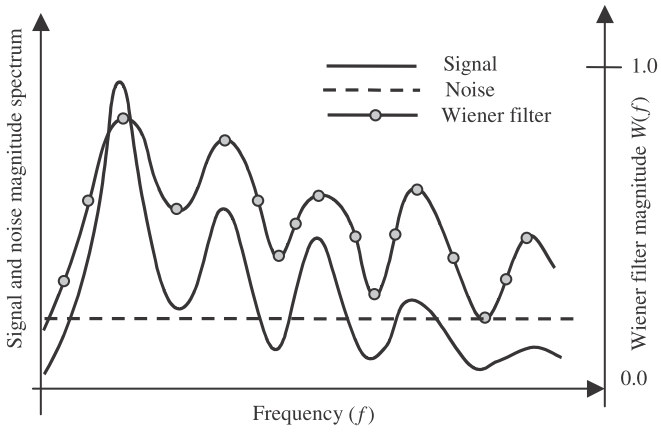
\includegraphics[scale=.4]{graph/Wiener}
        \end{figure}
 	\end{frame}

	\begin{frame}{denoising}{Wiener filter discussion 2/2}
      \vspace{-5mm} \begin{eqnarray*}
            W(\jom) &=& \frac{S_\mathrm{XX}(\jom)}{{S}_\mathrm{XX}(\jom) + {S}_\mathrm{NN}(\jom)}\\
            \pause
            &=& \frac{SNR(\omega)}{SNR(\omega) + 1}
        \end{eqnarray*}
        \smallskip
        $0\leq W(\jom)\leq 1$
        
        \vspace{-3mm}
        \begin{columns}
        \column{.6\textwidth}
        \begin{itemize}
            \item   limiting case 1: noise free
                \begin{eqnarray*}
                    SNR(\omega) &=& \infty\\
                    \pause
                    \Rightarrow  
                    W(\jom) &\rightarrow & 1
                \end{eqnarray*}
            \item   limiting case 2: extr. noisy
                \begin{eqnarray*}
                    SNR(\omega) &=& 0\\
                    \pause
                    \Rightarrow  
                    W(\jom) &\rightarrow & 0
                \end{eqnarray*}
        \end{itemize}
        \column{.4\textwidth}
        \begin{figure}
            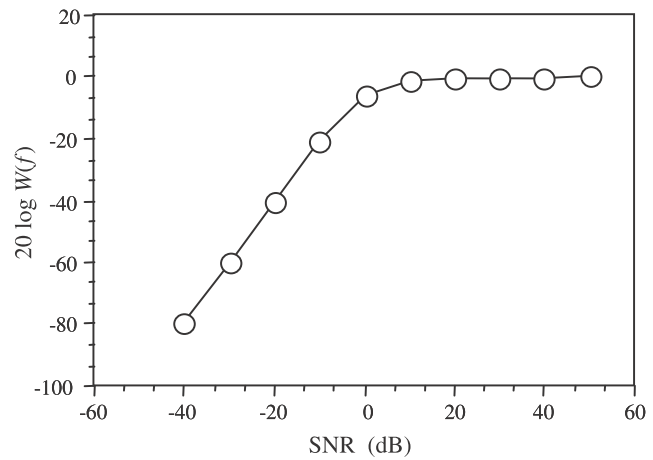
\includegraphics[scale=.3]{graph/WienerSNR}
        \end{figure}
        \end{columns}
 	\end{frame}

	\begin{frame}{denoising}{Wiener filter question}
        \question{How to estimate the noise spectrum}
        
        \begin{itemize}
            \item   user input: noise fingerprint
            \item   estimate from signal through, e.g., 
                \begin{itemize}
                    \item non-real-time: pause detection and automatic noise fingerprint selection
                    \item real-time: prediction error with smoothing constraints
                \end{itemize}
        \end{itemize}
	\end{frame}

\section{Spectral Subtraction}
 \setbeamercovered{invisible}
	\begin{frame}{denoising}{Spectral Subtraction}
        \begin{itemize}
            \item[] \textbf{idea}: Why not subtract the noise spectrum from the signal spectrum?
        \end{itemize}
        \begin{eqnarray*}
            |\hat{X}(\jom)|^2 &=& |Y(\jom)|^2 - |N(\jom)|^2\\
            &=& H(\jom)\cdot |Y(\jom)|^2\\
        \end{eqnarray*}
            \bigskip
            \pause
        \begin{eqnarray*}
            \Rightarrow H &=& 1-\frac{|N(\jom)|^2}{|Y(\jom)|^2}\\
            &=& \frac{|Y(\jom)|^2-|N(\jom)|^2}{|Y(\jom)|^2}
        \end{eqnarray*}
        \pause
        spectral subtraction identical to  Wiener filter when the power density spectrum estimates approach the ensemble means
	\end{frame}
	
%\section{summary}
		%\begin{frame}{summary}{denoising}
 		%\end{frame}

\end{document}

